\chapter{Sviluppo}
In questo capitolo verrà descritto il processo di sviluppo
seguito per l'implementazione di \pygfa, analizzandone le
fasi principali, descrivendo i problemi incontrati e come sono stati
affrontati.

\section{Processo}
Lo scopo di \pygfa è quello di fornire un ambiente per lo sviluppo
di applicativi in grado di analizzare e manipolare file GFA. Non
è pertanto un prodotto finito, con casi d'uso definiti e risultati attesi
con cui è possibile confrontare i risultati. Non si è ritenuto appropriato,
di conseguenza, seguire un processo di sviluppo con fasi di analisi
e pianificazione profonde, che con il mutare dei requisti (per la
maggior parte non definiti fin dall'inizio) avrebbero potuto
compromettere la struttura del sistema. Un altro fattore da
tenere in considerazione è che le mie conoscenze sul significato
che i dati contenuti nei file GFA e le considerazioni che si potevano dedurre
da esse sono cresciute con lo sviluppo del sistema stesso. Perciò un'analisi,
anche se non approfondita, non poteva essere svolta a priori; poiché
avrebbe potenzialmente comportato una serie di ritardi
nello sviluppo del progetto dovute allo studio dei concetti biologici
che avrebbe richiesto diverso tempo.


Per questi motivi, il processo di sviluppo che si è deciso di utilizzare è di \emph{extreme}
\emph{programming}; con fasi di analisi e pianificazione molto veloci,
dando priorità all'implementazione delle parti essenziali del sistema aventi
maggior priorità per poi ripetere il procedimento con l'evolversi dei
requisiti e delle funzionalità richieste, cercando di avere un riscontro
costante con i clienti finali (in questo caso i referenti della tesi).

Affiancata alla parte di implementazione si è svolta la parte di testing,
che purtroppo non si è riusciti a condurre esattamente nella forma di Test Driven
Development, ma alla quale è stata data comunque una priorità molto alta
sia per la verifica delle funzionalità dei metodi, che per la verifica della
presenza di errori nel codice, che nel contesto di un linguaggio non compilato,
quale è il Python, risulta una pratica molto importante per garantire il
corretto funzionamento del programma.

Nel complesso si è riusciti a seguire abbastanza rigorosamente questi cicli
di pianificazione veloce, implementazione e test; procedendo al termine
di ogni ciclo con una fase di refactoring del codice e di miglioramento
della documentazione presente in esso, avvalendosi di Pylint per individuare
quelle porzioni di codice che era possibile migliorare.

\subsection{Fasi di sviluppo}
La rappresentazione delle informazioni contenute nei file GFA subisce
diverse trasformazioni prima di giungere come dato di un nodo, arco o
sottografo presente in un oggetto grafo GFA. L' iniziale rappresentazione
testuale di ogni linea viene rappresentata da una classe che ne indica
il tipo e i valori dei campi che contiene. Successivamente le linee
vengono convertite in archi, nodi o sottografi e infine nodi e archi
vengono rappresentati mediante dizionari Python, una volta inseriti
effettivamente nel grafo. Quest'ultima trasformazione è stata
adottata per uniformarsi al trattamento dei dati di un grafo in modo analogo
al modo in cui NetworkX li gestisce, garantendo una facilità di accesso
alle informazioni ed evitando che l'utente finale debba adattarsi ad un
nuovo modo di operare.

\'E possibile suddividere lo sviluppo di \pygfa in tre fasi principali:
\begin{itemize}
	\item sviluppo del parser;
	\item progettazione delle classi di astrazione dei dati GFA;
	\item sviluppo della classe del grafo GFA e delle operazioni che è
		possibile eseguire su di esso.
\end{itemize}
\captionsetup{justification=centering}
\begin{figure}[h]
	\centering
	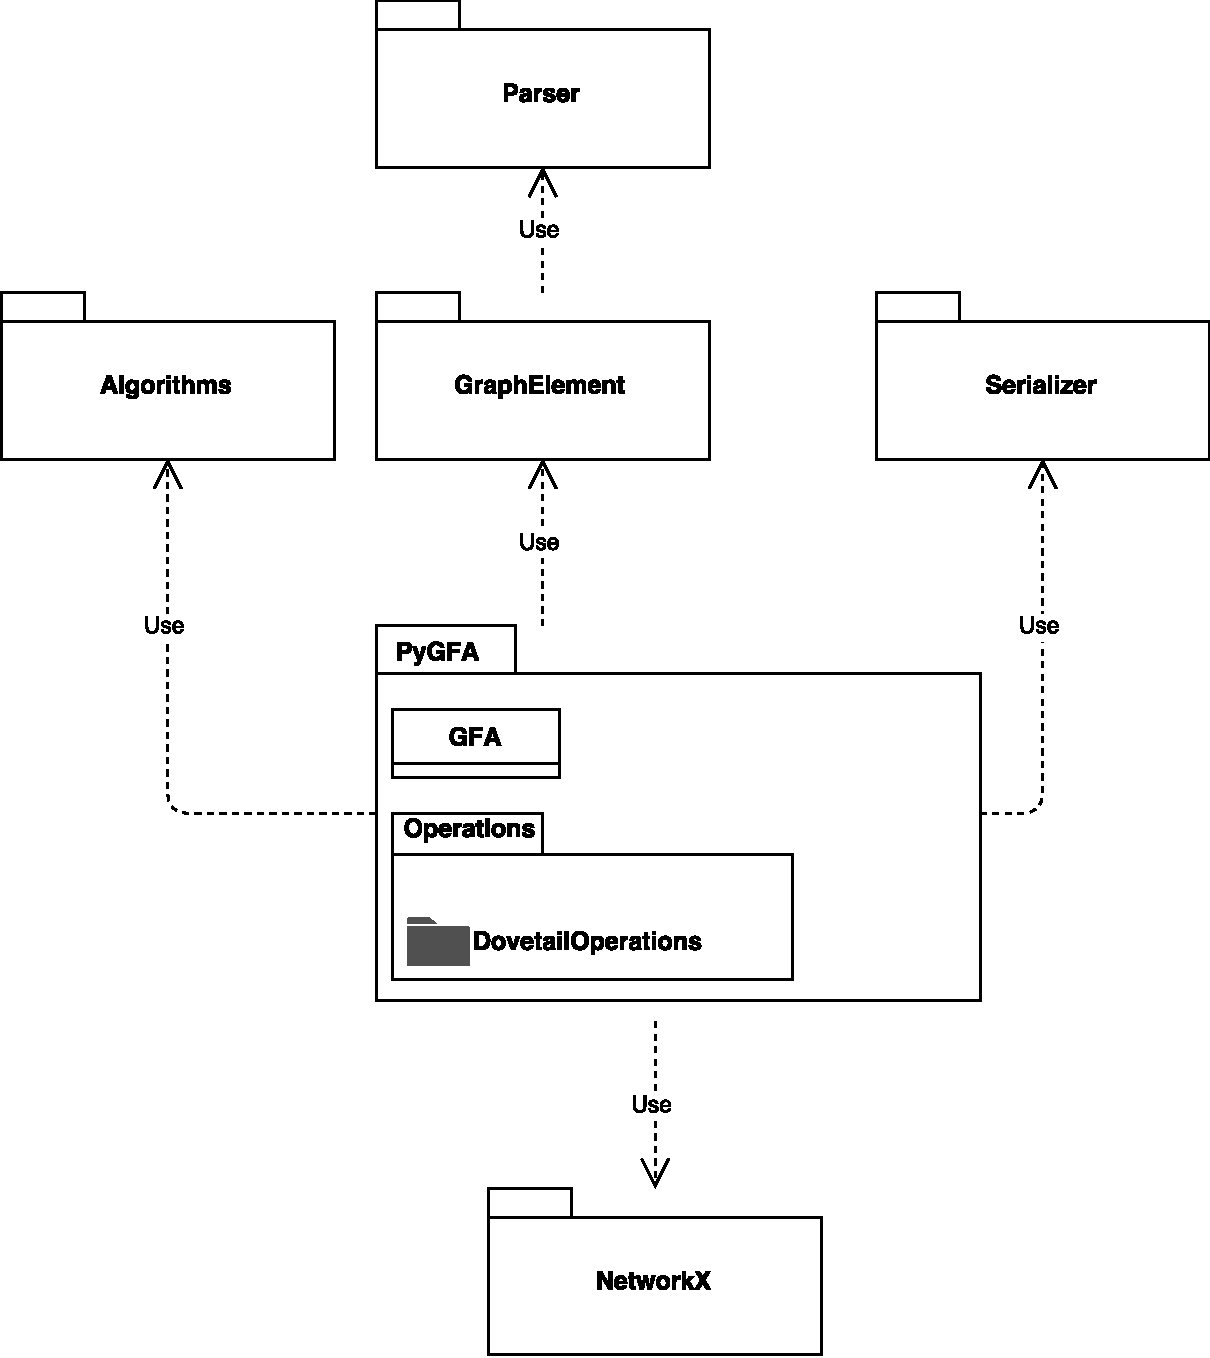
\includegraphics[scale=0.5]{package_diagram}
	\caption[Diagramma dei package]{Diagramma dei package di \pygfa.}
\end{figure}
\captionsetup{justification=justified}

Il parser si occupa di leggere le linee di un file GFA, di verificare la correttezza
sintattica dei suoi campi e di rappresentarne le informazioni mediante una classe
specifica per ogni tipo di linea.

Nella seconda fase si sono analizzate le linee delle due specifiche e si
è stabilito come attribuire ad ogni linea un ruolo che potesse essere di
nodo, arco o sottografo del grafo GFA finale. Gli attributi delle classi
del grafo astraggono gli attributi delle linee delle specifiche, 
di conseguenza è stata necessaria
una pianificazione dell'assegnamento degli attributi delle linee ad
attributi degli elementi del grafo.

Nella fase finale si è sviluppata la classe del grafo GFA fornendo
metodi di inserimento, accesso ed eliminazione sui singoli elementi che
lo compongono e aggiungendo le interfacce agli algoritmi forniti da Networkx
per eseguire le operazioni sui dati GFA.

\section{Fase1: sviluppo del parser}
Per la scrittura del parser si è seguito un approccio \emph{bottom-up},
sviluppando dapprima le classi rappresentanti i campi,
che sono presenti in ogni linea, 
e successivamente descrivendo con una classe ciascun tipo
di linea presente nelle specifiche.

Il parser effettua solo un controllo sintattico sulle informazioni dei file
al fine di garantire una corretta gestione delle informazioni da parte
della libreria; non verifica eventuali incongruenze tra le informazioni
presenti. Per questo motivo si suppone che il file GFA che viene fornito
sia stato già validato da un punto di vista di namespace degli elementi
e di coerenza delle informazioni (per esempio il riutilizzo di un identificativo
già utilizzato da un altro elemento o riferimenti a elementi
che non vengono definiti).

Ogni campo di ogni linea, in entrambe le specifiche, può essere descritto
da un \emph{espressione regolare}. Per questo motivo è stato
implementato un modulo Python per la validazione di tutti i campi definiti
dalle specifiche, associando un nome ad ogni espressione e creando un metodo
\texttt{is\_valid} che, data una stringa e il nome del tipo di un campo,
verifica che la stringa rispetti l'espressione regolare indicata dal nome
del campo fornito.
Per rappresentare i campi delle linee sono state create due classi,
\texttt{Field} e \texttt{OptField}; la prima
descrive i campi obbligatori, per i quali non viene specificato
esplicitamente il tipo di dato che contengono; la seconda
descrive i campi opzionali per i quali sono forniti
nome (il tag), tipo e valore. Mentre nei campi opzionali
è possibile, fin dall'instanziazione dell'oggetto, effettuare una validazione
sul contenuto, sui campi obbligatori non è possibile, in quanto
la tipologia del loro contenuto assume valore solo nel contesto
della linea cui appartengono.

Successivamente si è modellata la classe \texttt{Line} dalla quale
derivano le classi rappresentanti le altre linee. Questa classe
racchiude due campi: \texttt{PREDEFINED\_OPTFIELDS}
e \texttt{REQUIRED\_FIELDS} che racchiudono i campi opzionali che
ogni linea può contenere e i campi obbligatori che necessita, rispettivamente.
Inoltre questa classe possiede i metodi di aggiunta e rimozione dei campi,
assicurandosi di validare il contenuto dei campi obbligatori nel contesto
di ciascuna linea. Le altre classi, derivando da questa, devono
ridefinire i propri campi opzionali predefiniti e i campi obbligatori oltre
a indicare un metodo per convertire una stringa
nel corrispettivo oggetto che la rappresenta, condividendo la stessa
logica di manipolazione e validazione dei campi che viene riutilizzata
grazie al \emph{polimorfismo}.

\captionsetup{justification=centering}
\begin{figure}[h]
	\centering
	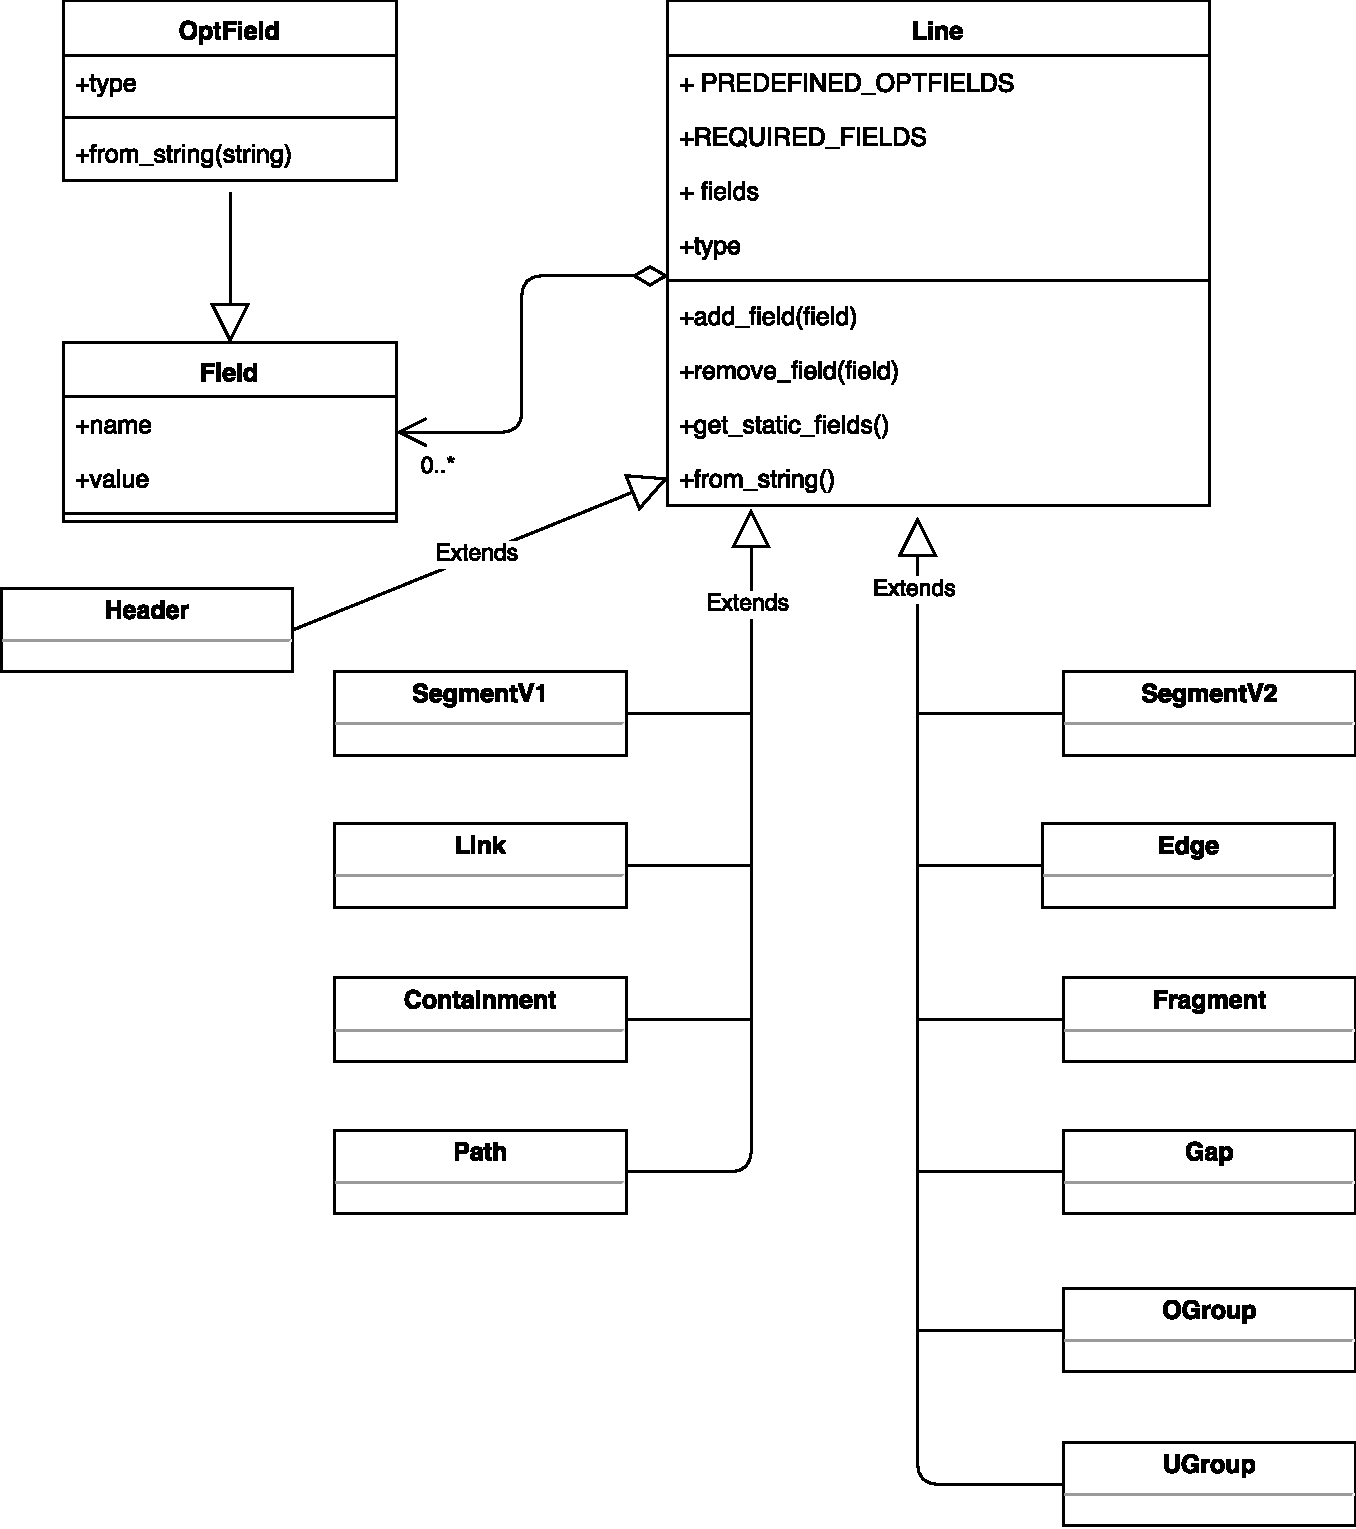
\includegraphics[scale=0.5]{parser_class_diagram}
	\caption[Diagramma delle classi del package parser]{Diagramma delle classi usate dal parser.}
\end{figure}
\captionsetup{justification=justified}
\clearpage

\section{Fase2: astrazione dei dati}
In questa fase sono state analizzate le singole informazioni presenti
nelle linee di entrambe le specifiche, evidenziandone gli aspetti simili al
fine di giungere ad una loro rappresentazione generalizzata per mezzo di tre
entità: \emph{Nodo}, \emph{Arco}, \emph{Sottografo}.

Ciascuna linea GFA può essere facilmente associata ad uno di questi tre
elementi. Nonostante sia possibile estendere GFA2 con nuovi tipi di linee, è bene notare
che questo lavoro di assegnazione di un ruolo ad ogni linea limita questa funzionalità
della specifica, in quanto sarebbe necessario capire il ruolo che queste nuove
linee possono ricoprire nei grafi di assemblaggio e ridefinire i meccanismi con
cui \pygfa riesce a manipolare queste nuove informazioni. \'E comunque possibile,
vista la mancanza dei concetti di visibilità privata del linguaggio, andare ad inserire
queste informazioni direttamente al grafo NetworkX che sta alla base dell'oggetto grafo
GFA, ma non è possibile garantire la consistenza delle operazioni che è possibile
effettuare usando la libreria.

Una sequenza costituisce il principale tipo di informazione cui si
è interessati, più sequenze sono in relazione da una serie di collegamenti descritti
dalle specifiche. Perciò possiamo attribuire alle sequenze (quindi alle linee Segment)
il ruolo di nodi.
La linea di header non contiene di per se informazioni che è possibile rappresentare
su di un grafo. Al momento \pygfa non modella le informazioni che possono essere
descritte dalle linee di header.

Tutte quelle linee che vedono come protagoniste due sequenze possono essere
considerate come degli archi che collegano due nodi $u$ e $v$. Appartengono
a tale insieme le linee di link, containment, edge, fragment e gap.

Le linee rimanenti: path, ogroup e ugroup, rappresentano tutte un insieme
(ordinato o meno) di nodi e archi che descrivono un sottografo composto
dagli elementi del file GFA; di conseguenza tali linee vengono considerate come
dei sottografi.

Visto che GFA2 è un superset di GFA1, si è analizzato come sarebbe stato
possibile rappresentare ciascuna linea di GFA1 nel corrispettivo elemento
di GFA2, capendo in questo modo gli attributi che ciascuna delle classi (Nodo, Arco
e Sottografo) avrebbe dovuto contenere per modellare quelle informazioni.
Terminato il confronto delle linee di GFA1 si sono aggiunte quelle
informazioni delle linee di GFA2 che non erano state prese in considerazione
(poiché non rappresentate) e le si sono andate ad aggiungere come attributi
aggiuntivi delle classi rappresentanti gli elementi del grafo.
Le informazioni che diventeranno attributi espliciti delle classi sono date
esclusivamente dai campi obbligatori di ciascuna linea, per entrambe le
classi i dati provenienti da campi opzionali verranno memorizzate
all'interno di un dizionario Python e indicate da un unico campo
\texttt{opt\_fields}; si noti che nonostante il nome, i campi contenuti
non sono (solamente) riferimenti ai campi opzionali delle specifiche,
ma si riferiscono ad una qualsiasi informazione
che l'utente vuole aggiungere all'elemento.

Di seguito verrà elencato ciascun campo di ogni linea, la relativa rappresentazione
in GFA2 e la scelta di come si è deciso di modellare tale campo nell'elemento
del grafo corrispondente. Per i nomi dei campi si farà riferimento alla nomenclatura
utilizzata dalla specifica per indicare ciascun campo, si noti
che alcuni nomi potrebbero subire variazioni in quanto la specifica è attivamente
in sviluppo e subisce continui cambiamenti. In questa tabella si fa riferimento
al nome dei campi così come si sono presentati al momento della fase dello
sviluppo.
Eventuali cambiamenti apportati negli ultimi periodi (entro la data indicata
dalla bibliografia) saranno indicati a piè pagina.

\subsection{Attributi della classe Nodo}
La classe nodo rispecchia senza aggiungere altre complicazioni
i campi descritti dalla linea GFA2 Segment.
Il campo \texttt{slen} che descrive la lunghezza della linea, nel
caso di GFA1, viene recuperato dal campo opzionale \texttt{LN};
nel caso non fosse specificato si cerca di ricavare tale valore
dalla sequenza stessa, calcolandone la lunghezza. Se la
sequenza non è specificata il dato assume valore \texttt{None}, per
indicare la mancanza di tale informazione.
\noindent
\begin{table}[h]
	\rowcolors{1}{white}{lightgray}
	\begin{tabularx}{\textwidth}{ | X | X | X |}
		\hline
		\textbf{Campo GFA1}	&	\textbf{Campo GFA2}	&	\textbf{Attributo nodo}\\
		Name				&	sid					&	nid (node id)\\
		Sequence				&	sequence				&	sequence\\
		Campo opzionale LN, lunghezza linea o \mbox{\textbf{None}}	&	slen	& slen\\
		\hline
	\end{tabularx}
	\caption{Tabella di analisi degli attributi del nodo.}
	\label{tab:node-analysis}
\end{table}


\subsection{Attributi della classe Arco}
Per determinare gli attributi della classe arco si sono dovuti analizzare i campi
di tutte le linee che potessero essere riconducibili ad un arco del grafo.

La prima linea da analizzare è stata la linaa Link della specifica GFA1, la quale è
possibile ricondurla alla linea Edge di GFA2. Si nota dalla tabella \ref{tab:link-analysis}
l'esistenza di una corrispondenza uno a uno tra i campi della linea Link e quelli
della linea Edge. I campi della linea Edge contengono anche le posizioni
delle sequenze nelle quali si verifica l'overlap, ma tale informazione non è presente
nel Link di conseguenza questi quattro attributi dell'arco rappresentante un link
(beg1, end1, beg2 ed end2) saranno impostati a None.

\noindent
\begin{table}[h]
	\rowcolors{1}{white}{lightgray}
	\begin{tabularx}{\textwidth}{ | X | X | X |}
		\hline
		\textbf{Campo GFA1}	&	\textbf{Campo GFA2}			&	\textbf{Attributo arco}\\
		Campo opzionale ID o	\mbox{\textbf{None}}				&	eid					&	eid (edge id)\\
		From				&	sid1 (escludendo il segno)		&	from\_node\\
		From Orientation		&	segno di sid1					&	from\_orn\\
		To					&	sid2 (escludendo il segno)		&	to\_node\\
		To Orientation			&	segno di sid2					&	to\_orn\\
		Alignment				&	alignment						&	alignment\\
		\hline
	\end{tabularx}
	\caption{Tabella di analisi degli attributi della linea Link.}
	\label{tab:link-analysis}
\end{table}

Lo stesso comportamento è stato usato con la linea di Containment. In questo
caso però il campo relativo la posizione di inizio della sequenza contenuta non
è indicata nell'equivalente linea GFA2 Edge, e tale informazione
si è rivelata deducibile dalle posizioni di inizio e fine dell'overlap
indicata dal Edge stesso, di conseguenza a questa informazione è stata attribuita
una priorità minore e si è scelto di inserirlo come ulteriore campo opzionale dell'arco (chiamandolo
\texttt{pos}),
in modo da non perdere l'informazione nella fase di serializzazione
del grafo GFA in formato testuale.

Analizzando le altre linee rimanenti in GFA2 (Edge, Gap e Fragment), oltre agli attributi
necessari a rappresentare i campi di GFA1, si sono aggiunti gli attributi per
rappresentare l'inizio e la fine delle posizioni che coinvolgono l'overlap rispettivamente
per la sequenza di partenza e di arrivo, inoltre l'analisi sulle linee di Gap
ha richiesto l'aggiunta di attributi relativi la varianza e la distanza che questa linea
descrive. L'unica particolarità da evidenziare è la mancanza di un campo
analogo ad \texttt{eid} per la linea Fragment.

Si noti che le informazioni, con questo livello di astrazione, rendono difficile distinguere
le linee di Link, da quelle di Edge e di Fragment (le linee di Containment si distinguono
per la presenza del campo \texttt{pos} all'interno dei campi opzionali dell'arco mentre
quelle di Gap hanno sempre definiti gli attributi di varianza e distanza che le altre linee
hanno impostate a \textbf{None}). In questo caso la distinzione fra queste linee avviene avviene come
segue: gli Edge e i Link avranno il simbolo di asterisco come
identificativo nel caso l'informazione sia mancante,  mentre i Fragment
non hanno alcun campo che descrive un identificatore che li referenzia, perciò
il loro campo \texttt{eid} sarà None. Fatta questa distinzione, le linee di Edge se necessario
possono essere distinte da quelle di Link per la mancanza delle informazioni
circa le posizioni del overlap fra le sequenze che i Link descrivono.

In aggiunta agli attributi dei campi, si è deciso di aggiungere altre
tre informazioni per ogni.
Queste informazioni riguardano nello specifico i Link e gli Edge che
rappresentano un dovetail overlap (cioè quegli Edge che descrivono un Link).
Per questo tipo di archi viene impostato un attributo booleano \texttt{is\_dovetail}
che viene posto a vero e successivamente con i valori degli orientamenti
delle sequenze e delle posizioni dell'overlap (per gli Edge) vengono impostati
due campi \texttt{from\_segment\_end} e \texttt{to\_segment\_end} che indicano
l'estremità delle sequenze (``from'' e ``to'', rispettivamente) che vengono
prese in considerazione dall'overlap. Nel caso degli archi che non presentano
questa situazione, l'attributo \texttt{is\_dovetail} è impostato a falso e
gli attributi riguardanti le estremità sono posti a None.

Questa scelta ha permesso di andare ad effettuare tutta una serie di operazioni
sul grafo di notevole importanza ai fini dell'assemblaggio del genoma, visto che
le sovrapposizioni di dovetail rappresentano un continuum fra sequenze.
Se non si fosse adoperata questa soluzione il livello di astrazione introdotto da \pygfa
nella rappresentazione dei dati sarebbe stato troppo elevato e non avrebbe
permesso di usare efficacemente tutta una serie di operazioni che avrebbero
avuto senso solo per collegamenti di questo tipo.

